\section{Usuwanie konta}

Usuwanie kont klienta oraz wykonawcy okazało się bardziej skomplikowanym w implementacji, niż się tego spodziewano. Wymagało ono przeprowadzenia licznych operacji w bazie danych oraz dodatkowych założeń. Przyjęto, że usunięcie konta klienta pozostawi wszystkie dodane przez niego oceny i komentarze nienaruszone, aby inni mogli wciąż na nich bazować. Znikną one dopiero wraz z usunięciem wykonawcy. Pozostawiane są również wszystkie oferty klienta, ponieważ wykonawcy wciąż mogą mieć do nich dostęp. Są one usuwane dopiero, gdy obie strony go stracą. Z kolei zlecenia są usuwanie wtedy, gdy zarówno klient będący ich twórcą, jak i wszystkie zgłoszone oferty zostaną usunięte. W implementacji tych zależności pomogły funkcje wywoływane modyfikacją danych, dostępne w ramach Firebase Functions. 

\begin{figure}[ht]
  \captionsetup[subfigure]{justification=centering}
  \centering
  \begin{subfigure}[t]{0.32\textwidth}
    \centering
    \fbox{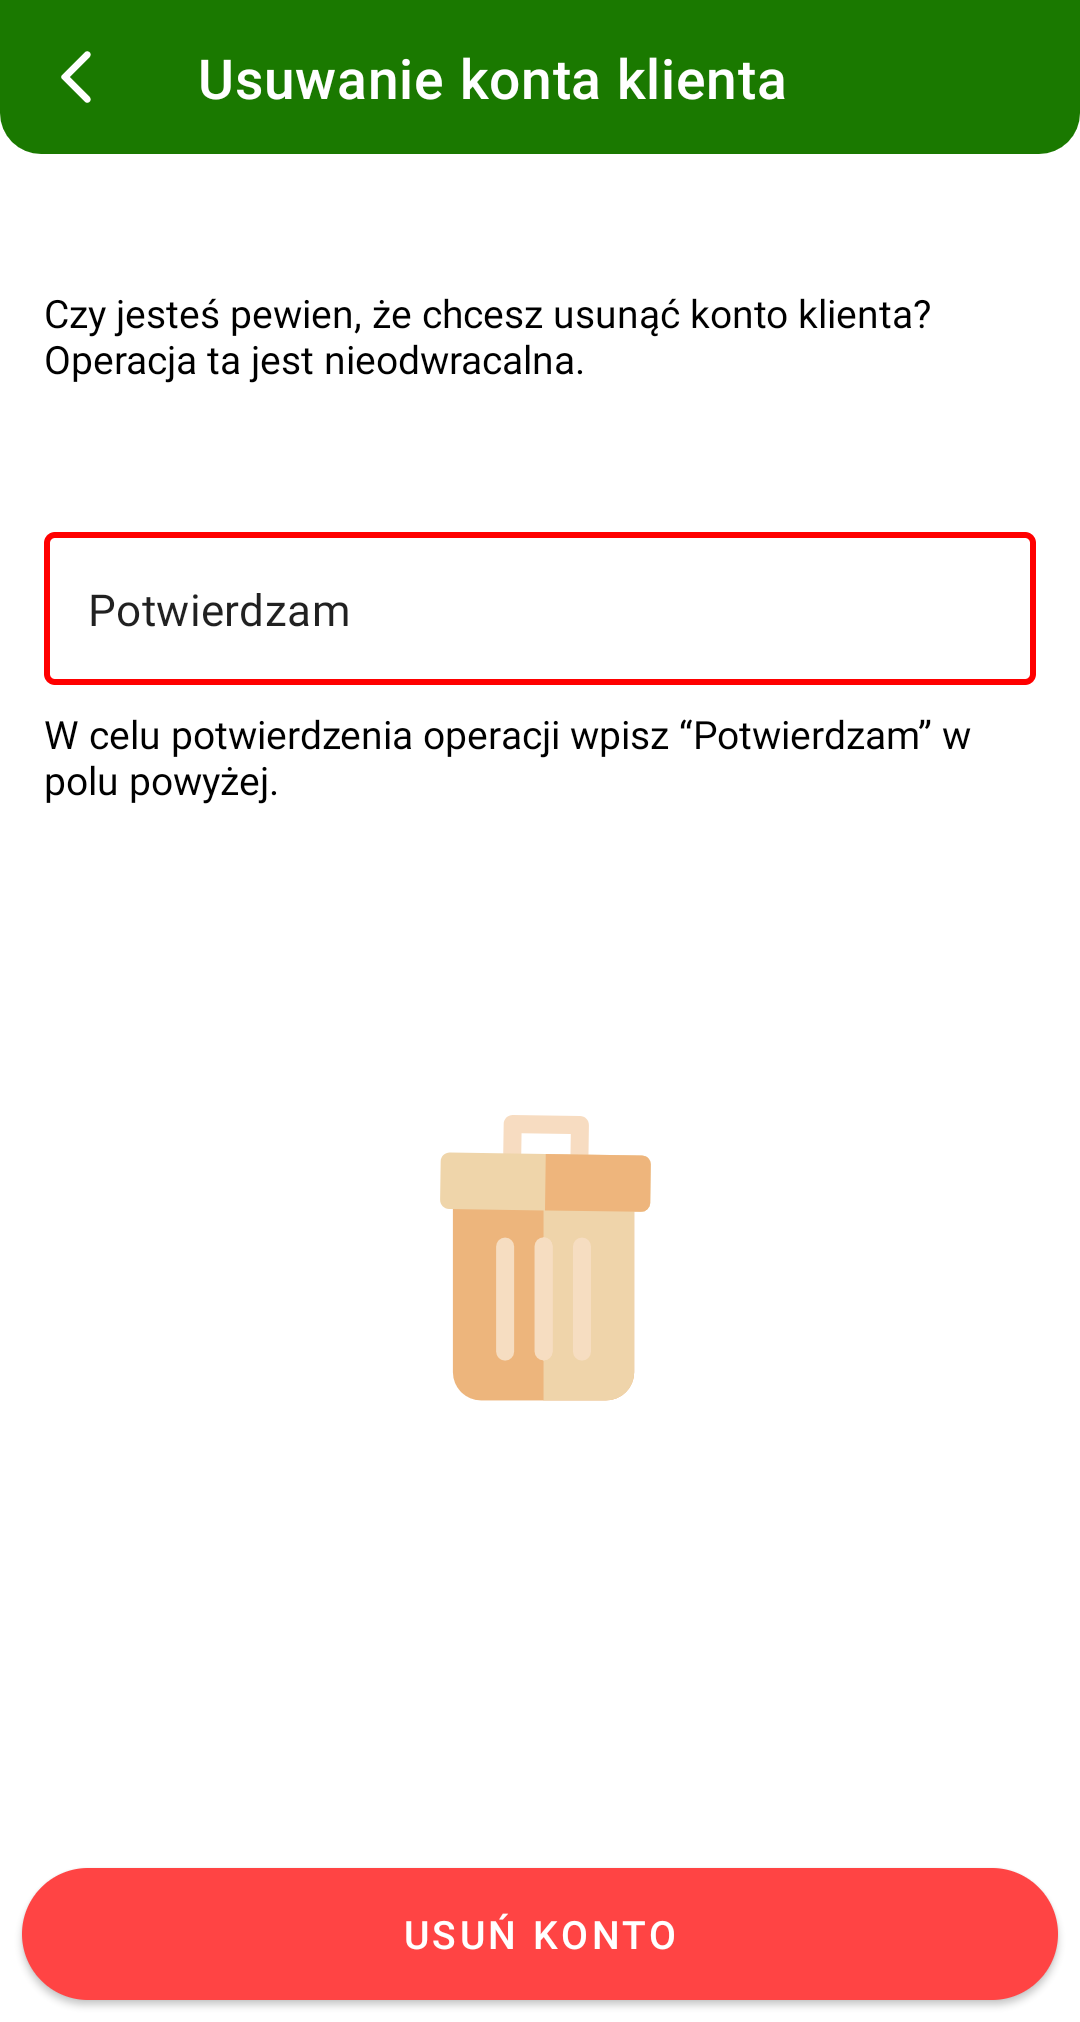
\includegraphics[width=0.97\linewidth]{screens/delete.png}}
    \caption{Ekran usuwania konta klienta}
  \end{subfigure}
  \begin{subfigure}[t]{0.32\textwidth}
    \centering
    \fbox{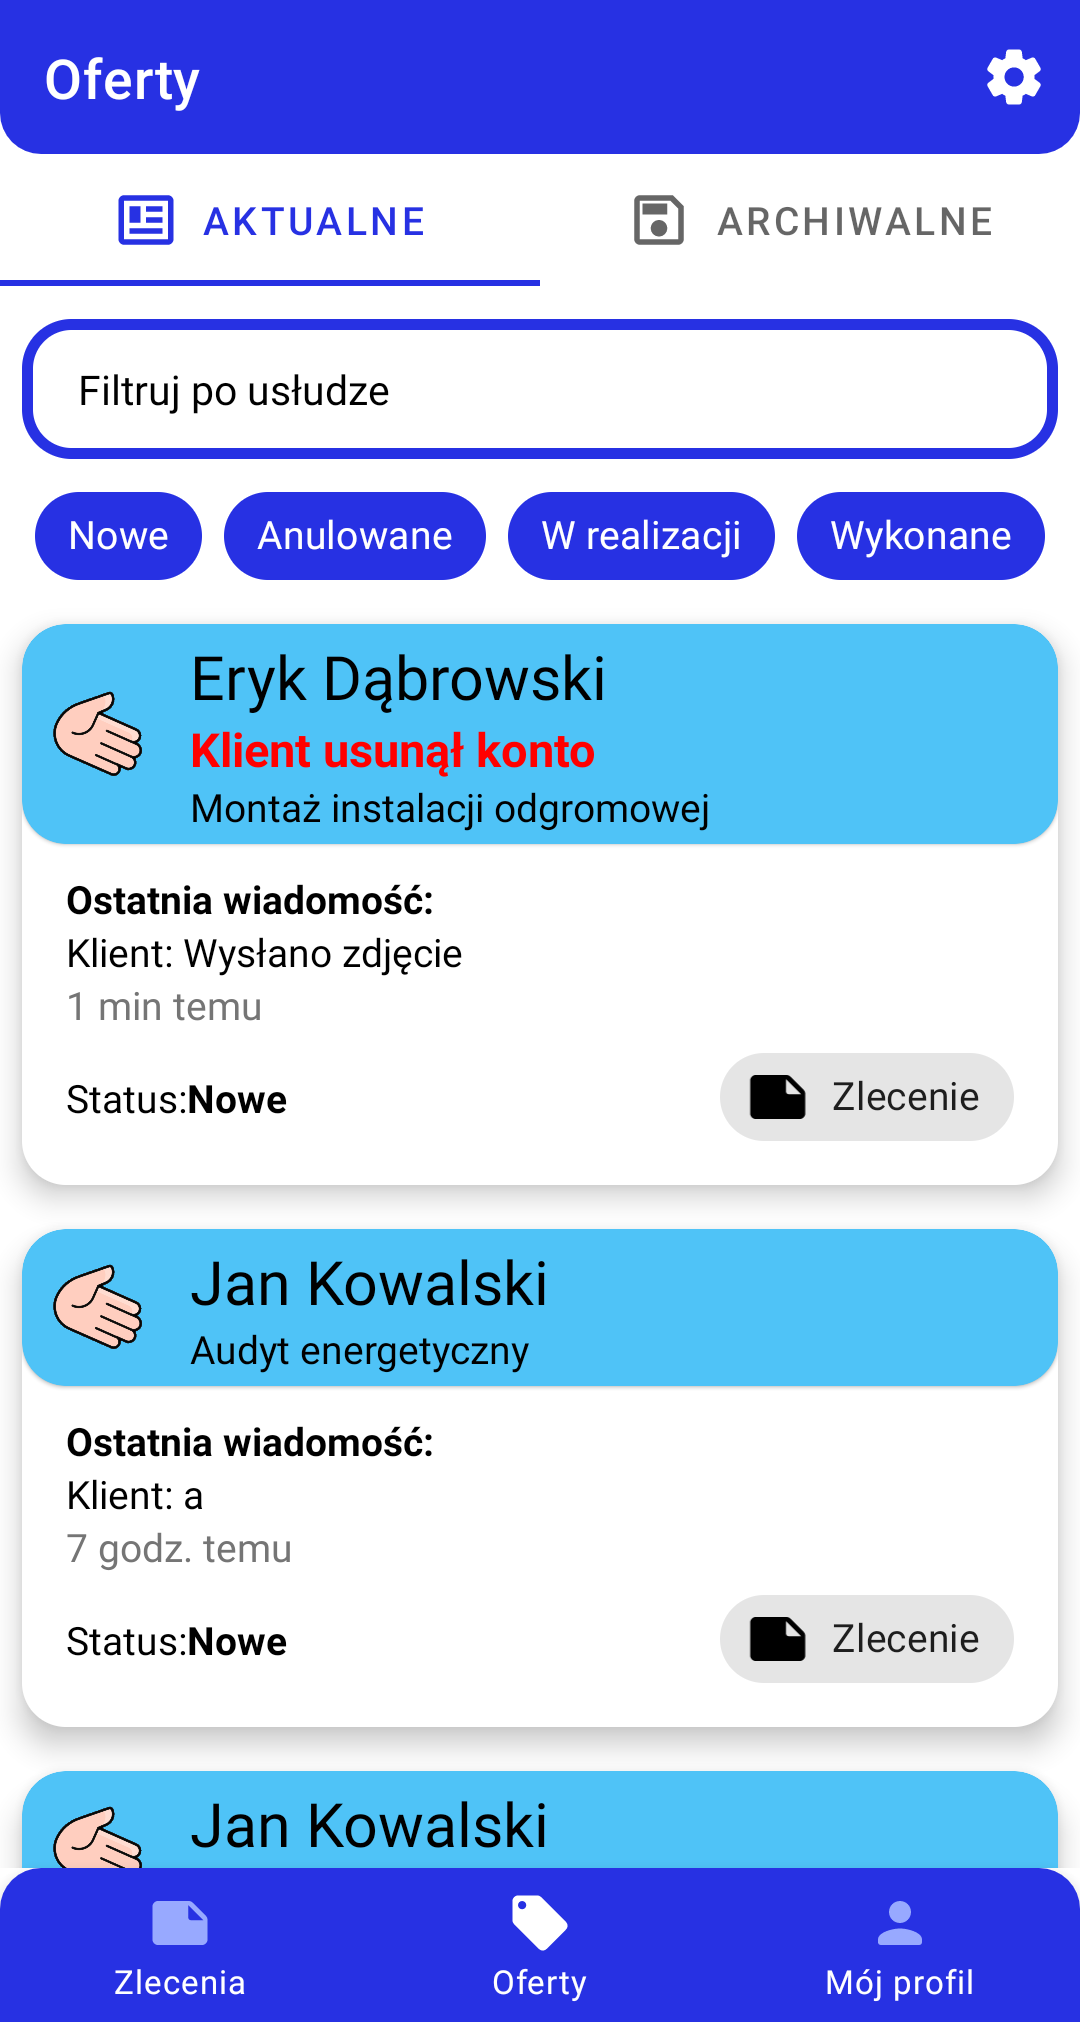
\includegraphics[width=0.97\linewidth]{screens/delete_offers.png}}
    \caption{Widok usuniętego klienta na liście ofert}
  \end{subfigure}
  \begin{subfigure}[t]{0.32\textwidth}
    \centering
    \fbox{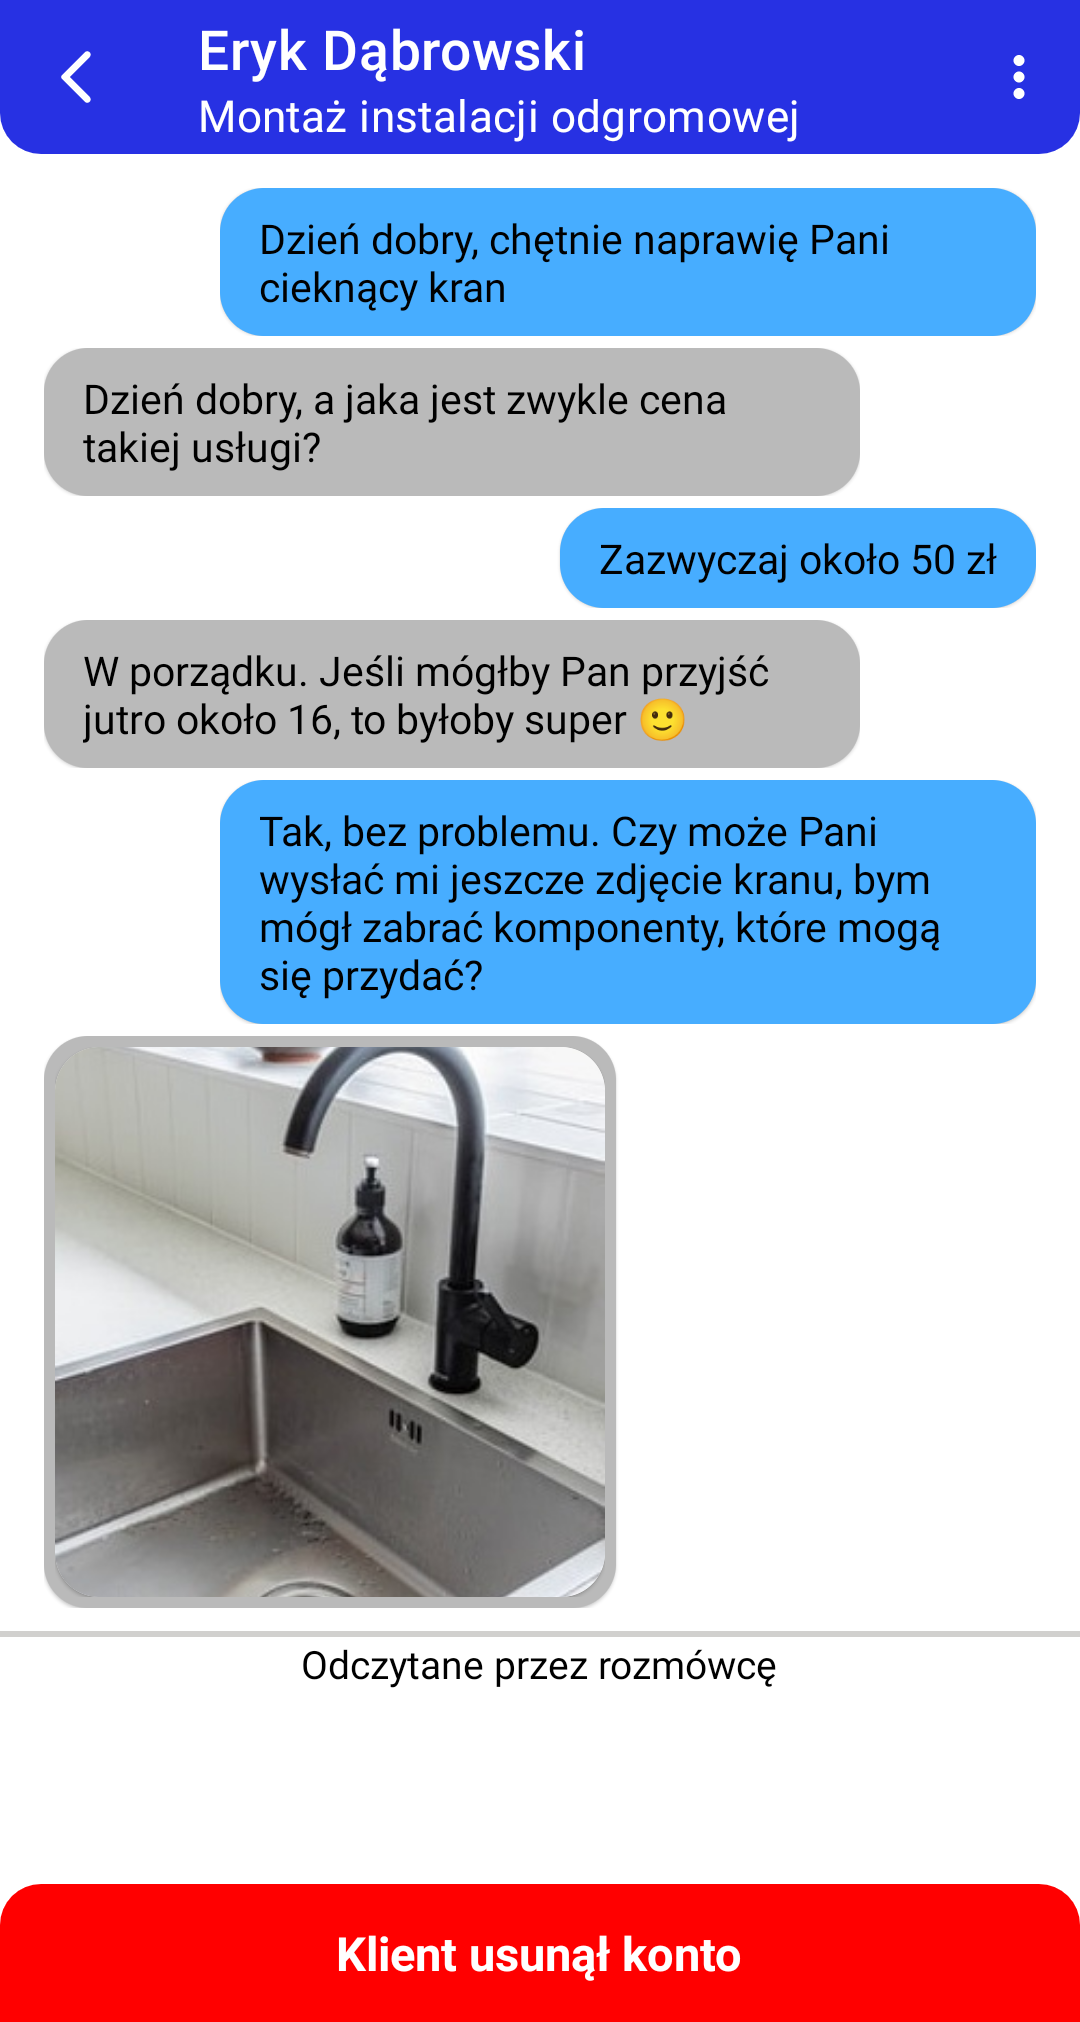
\includegraphics[width=0.97\linewidth]{screens/delete_offer.png}}
    \caption{Ekran chatu z usuniętym klientem}
  \end{subfigure}
  \caption{Ekrany związane z usuwaniem konta}
  \label{fig:delete}
\end{figure}

Na rysunku \ref{fig:delete} przedstawiono ekrany związane z usuwaniem konta przez klienta. Aby operacja mogła zostać wykonana użytkownik musi wpisać w polu tekstowym słowo \enquote{Potwierdzam}. Jest to zabezpieczenie przeciwko przypadkowemu i niechcianemu działaniu. Gdy konto zostanie usunięte, to użytkownicy, którzy wchodzili z nim wcześniej w interakcję zobaczą o tym powiadomienie przy odpowiedniej ofercie. Nie będą mieli od tej pory możliwości komunikacji z nim za pomocą chatu, chociaż przeglądanie historii wiadomości wciąż będzie dostępne.